\chapter[AI Component: Experiments and Evaluation]{AI Component: Experiments and~Evaluation}

\section*{Introduction}
\phantomsection
\addcontentsline{toc}{section}{Introduction}
This chapter constitutes the scientific core of the AI component. It presents the full experimental methodology, beginning with Exploratory Data Analysis (EDA) of the collected dataset, followed by the validation of the multimodal feature extraction pipeline. It then reports model training and evaluation results using regression metrics, learning curves, and SHAP explainability, in order to rigorously demonstrate the reliability of the Pre‑Posting Predictive Agent.

\section{Dataset Description and Data Collection}
To train the Pre-Posting Predictive Agent, a custom multimodal dataset was constructed, since no public dataset provides both raw short-form videos and their algorithmic reach metrics.

\begin{itemize}
    \item \textbf{Sources:} TikTok, YouTube Shorts, and Instagram Reels.
    \item \textbf{Collection Method:} Automated scraping using \texttt{yt-dlp} and platform-specific scripts to download both \texttt{.mp4} files and metadata.
    \item \textbf{Size and Format:} $\sim$1,100 raw videos stored as \texttt{.mp4}, accompanied by a unified metadata table (\texttt{all\_metadata.csv}) containing fields such as \texttt{video\_id}, \texttt{title}, \texttt{platform}, \texttt{duration\_seconds}, \texttt{views}, \texttt{upload\_date}, and \texttt{local\_video\_path}.
    \item \textbf{Multimodal Outputs:} Each video is processed into separate feature artifacts: 
    \begin{itemize}
        \item \textbf{Visual Embeddings:} CLIP vectors for hook and full video (\texttt{.npy} files).
        \item \textbf{Audio Features:} Librosa acoustic descriptors (RMS, tempo, MFCCs, silence ratio) saved as JSON.
        \item \textbf{Transcripts:} Whisper ASR output (hook + full transcript) stored as JSON.
        \item \textbf{Textual Embeddings:} SentenceTransformer vectors for combined title + transcript.
        \item \textbf{LLM Annotations:} Llama/Groq semantic labels (tone, hook type, scores), structured as JSON.
    \end{itemize}
    \item \textbf{Data Cleaning:} Duplicate \texttt{video\_id}s were removed prior to splitting to prevent leakage. Videos with corrupted audio or missing files were discarded, and silent videos were kept but labeled with empty transcripts.
\end{itemize}

% ══════════════════════════════════════════════════════════════
\section{Exploratory Data Analysis (EDA)}
% ══════════════════════════════════════════════════════════════
Before training, we conducted a rigorous EDA on the combined dataset of $\sim$1,100 short-form videos to understand the underlying statistical distributions and correlations.

\subsection{Target Variable Transformation}
Social media views naturally follow an exponential power-law distribution. Most videos receive very few views, while a small minority go massively viral. 

\begin{figure}[H]
    \centering
    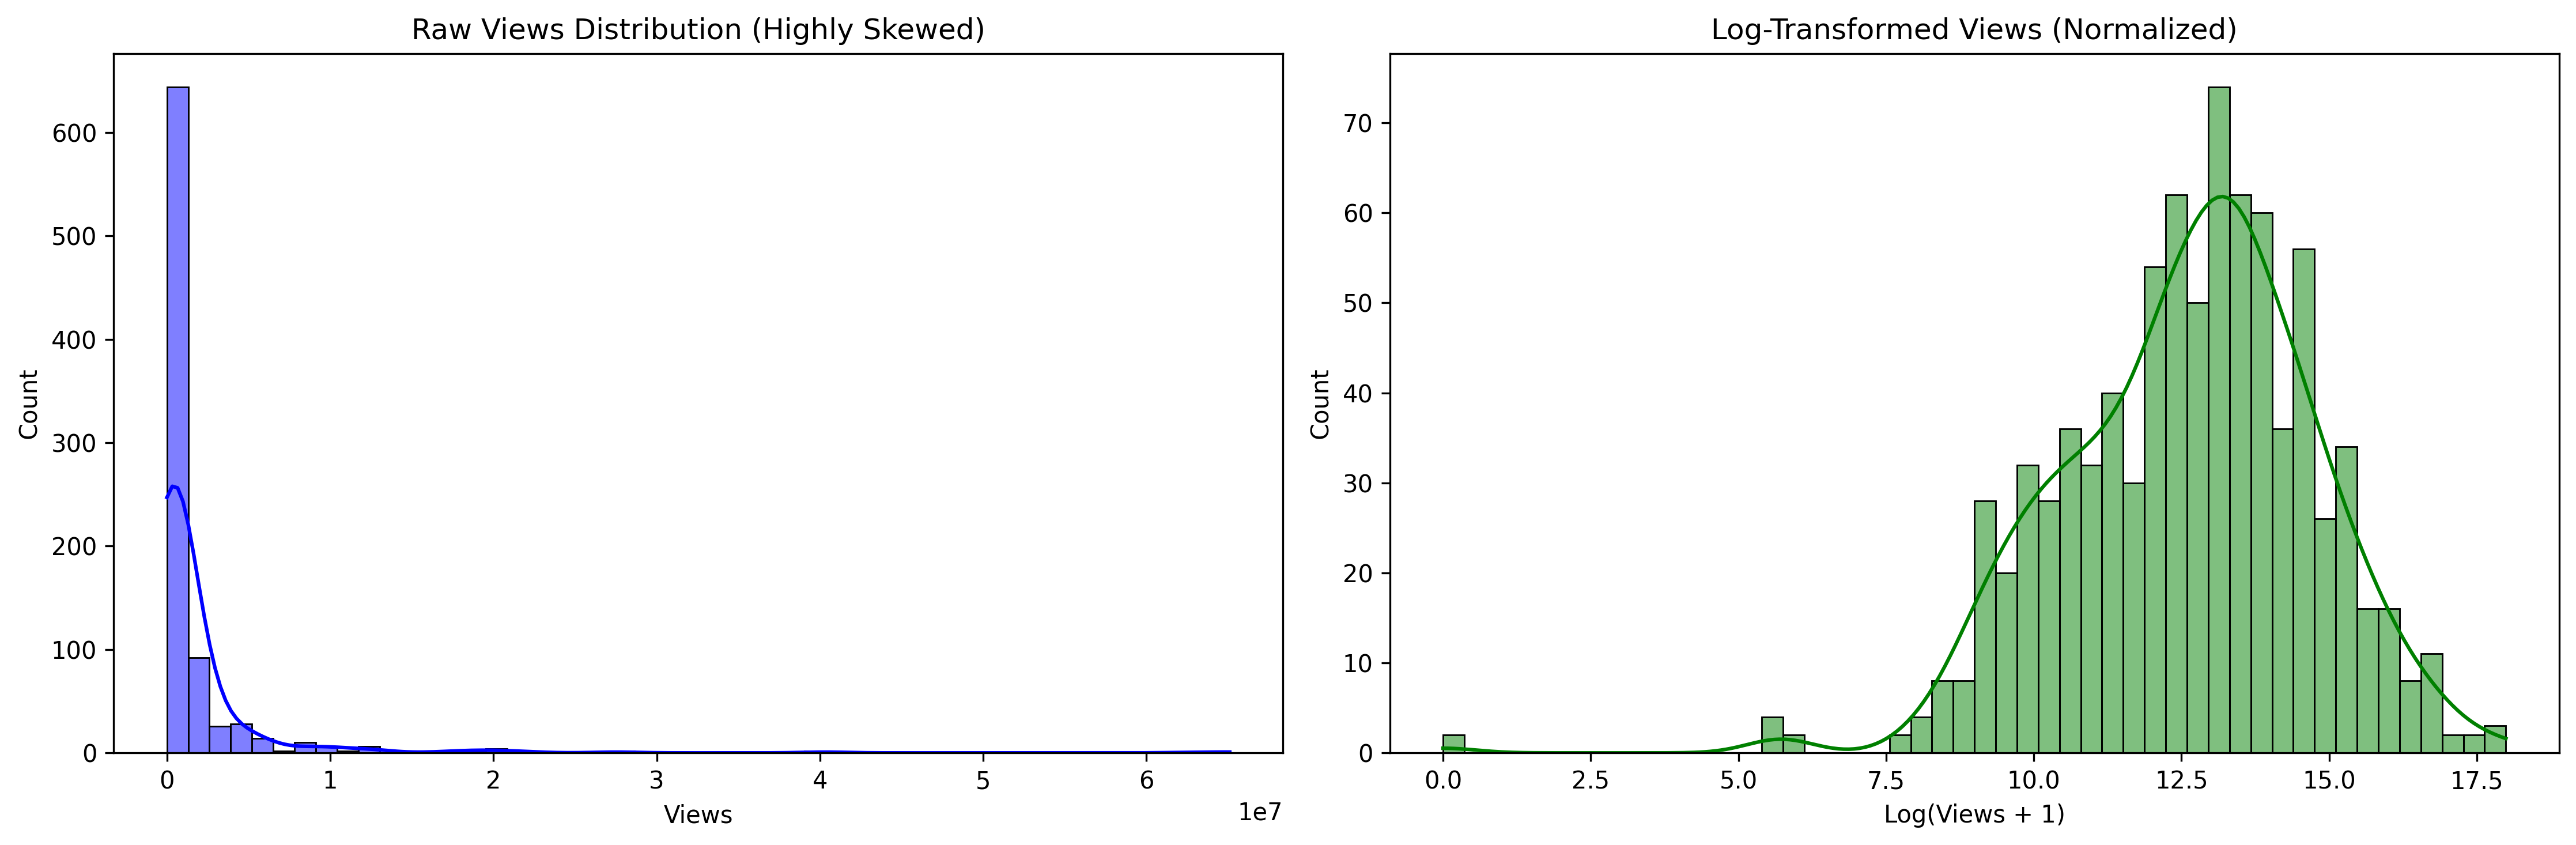
\includegraphics[width=0.9\textwidth]{images/target_distribution.png}
    \caption{Distribution of raw views (left) versus the Log-Transformed target variable (right).}
    \label{fig:eda_distribution}
\end{figure}

As observed in Figure \ref{fig:eda_distribution}, the raw view counts are heavily right-skewed. To prevent the regression model from being disproportionately penalized by these viral outliers, a logarithmic transformation (\texttt{numpy.log1p}) was applied. This successfully transformed the target variable (\texttt{log\_views}) into a Gaussian-like distribution, stabilizing the loss function during training.

\subsection{Feature Correlation Analysis}
To investigate linear relationships, we generated a Pearson Correlation Matrix comparing our extracted features against \texttt{log\_views}.

\begin{figure}[H]
    \centering
    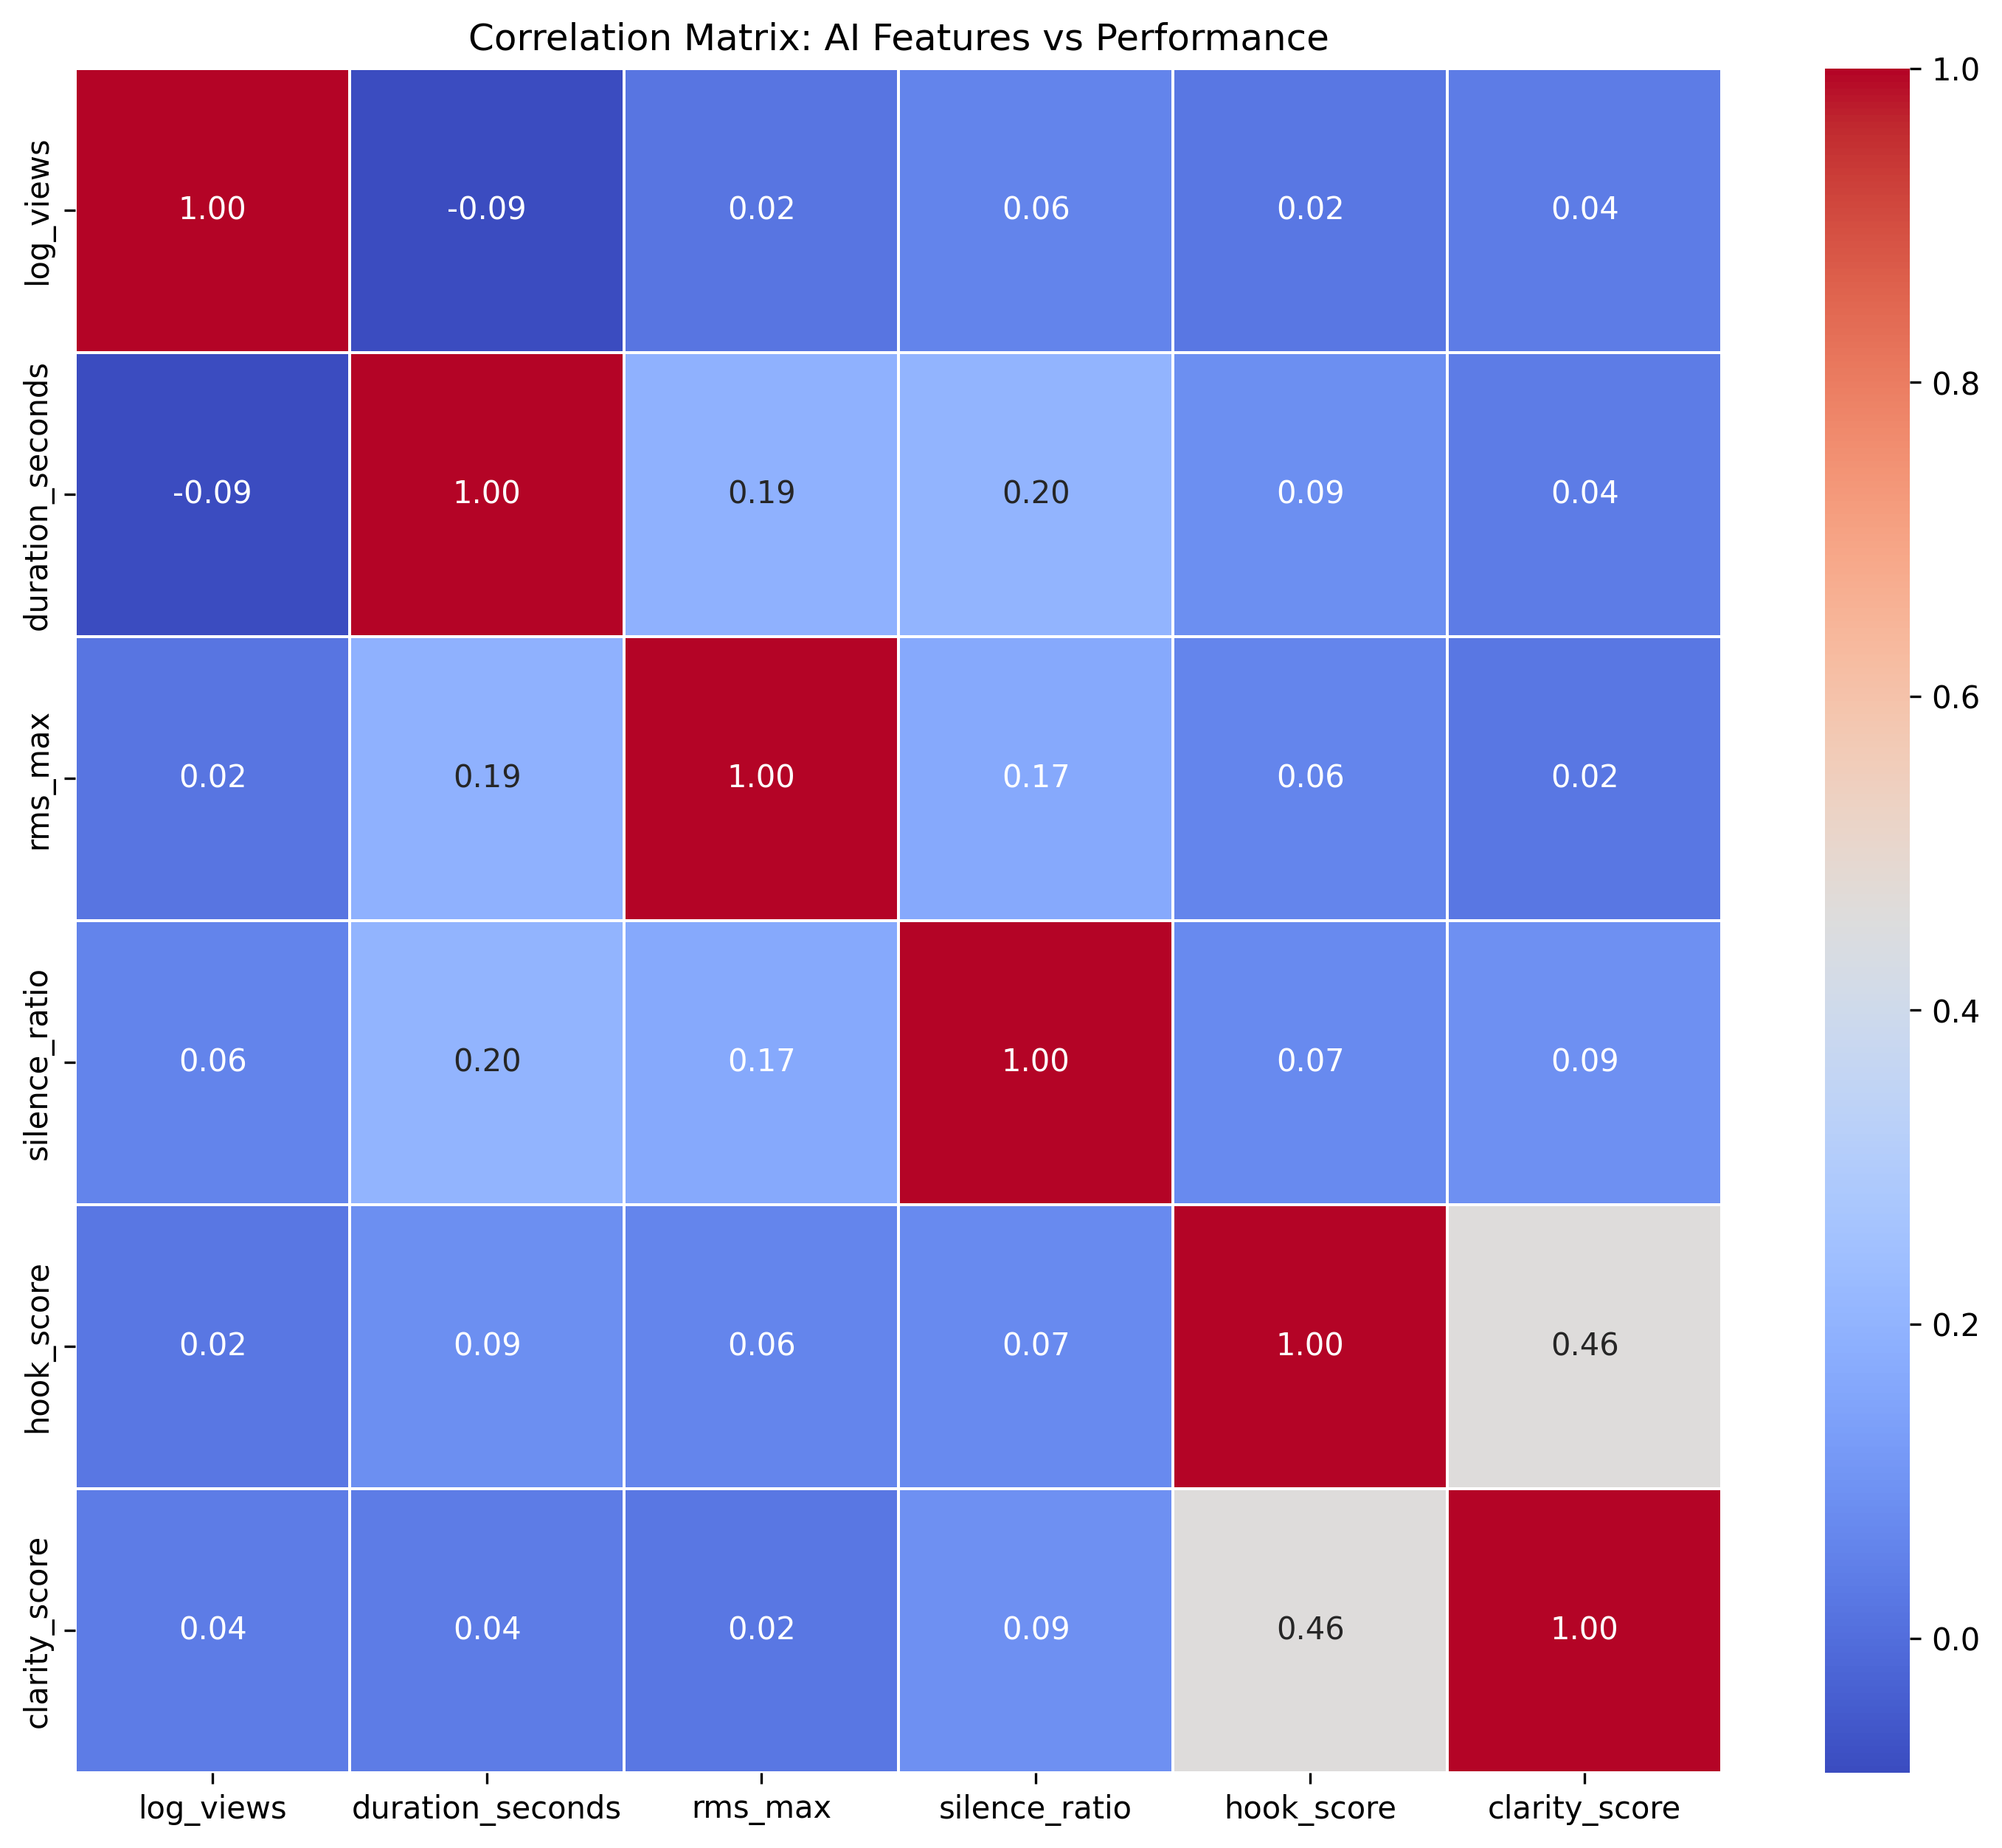
\includegraphics[width=0.4\textwidth]{images/correlation_matrix.png}
    \caption{Pearson Correlation Matrix of AI features vs algorithmic reach (\texttt{log\_views}).}
    \label{fig:eda_correlation}
\end{figure}

Figure \ref{fig:eda_correlation} reveals that no single feature has a strong linear correlation with \texttt{log\_views} (values hovering near zero). This critical finding proves that virality cannot be predicted using simple linear regression. Instead, it justifies our architectural decision to utilize XGBoost, a tree-based ensemble capable of mapping highly complex, non-linear interactions across multiple modalities.

% ══════════════════════════════════════════════════════════════
\section{Feature Extraction \& Dimensionality Reduction}
% ══════════════════════════════════════════════════════════════
The dataset is composed of raw \texttt{.mp4} videos and metadata, which cannot be used directly by machine learning models. Therefore, a dedicated multimodal extraction pipeline was designed to transform each video into structured numerical representations across visual, audio, and semantic modalities. This section details the extraction stages and provides visual evidence to validate the correctness and consistency of the resulting features.
\subsection{Acoustic Extraction (Librosa)}
The first three seconds of a video (the “Hook”) strongly influence viewer retention.\\  To capture these early‑stage acoustic signals, we extracted a short audio window and computed multiple low‑level descriptors using \texttt{librosa}. \\ 
These include RMS energy (loudness), zero‑crossing rate (signal roughness), spectral centroid and roll‑off (brightness), tempo (pacing), silence ratio (dead‑air detection), and MFCCs (timbre). Together, these features quantify pacing, clarity, and auditory intensity factors that are directly linked to a viewer’s decision to continue watching.

\begin{figure}[H]
    \centering
    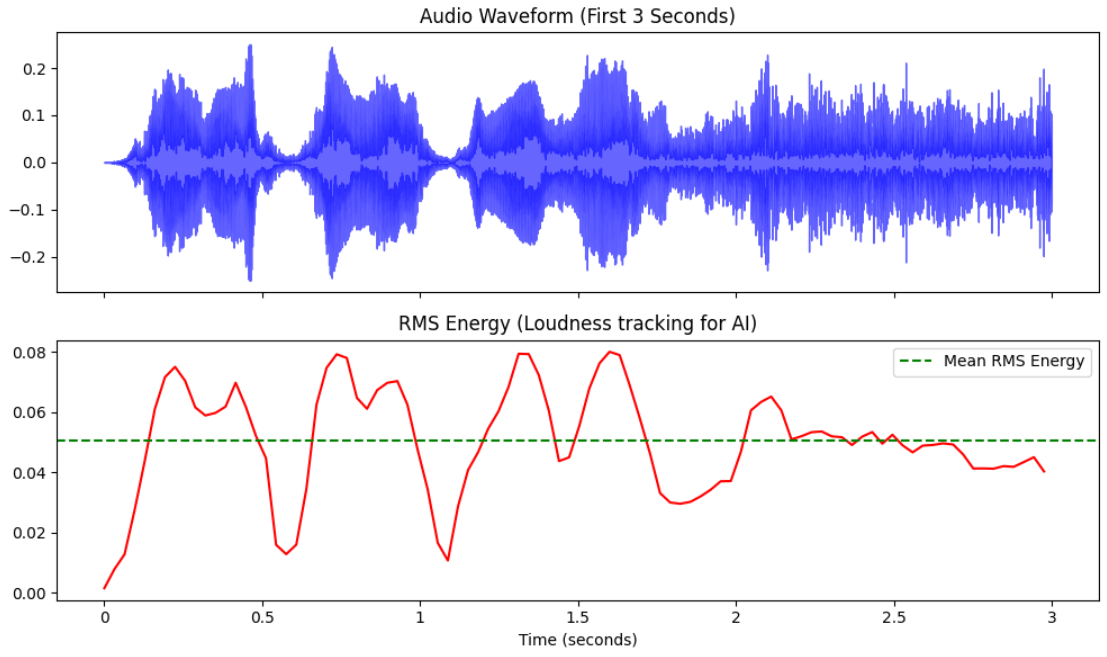
\includegraphics[width=0.8\textwidth]{images/acoustic_features.png}
    \caption{Acoustic feature extraction: Raw audio waveform and RMS Energy.}
    \label{fig:acoustic_features}
\end{figure}

 Figure \ref{fig:acoustic_features}  illustrates how the raw waveform is converted into short‑time energy. RMS energy captures the loudness envelope of the hook, which is critical for detecting silence, weak delivery, or abrupt drop‑offs. We define the \texttt{silence\_ratio} as the proportion of frames whose energy falls below a fixed threshold, enabling the model to quantify “dead air.” This metric is especially important in short‑form content, where low energy in the first seconds strongly predicts early viewer drop‑off.

\begin{figure}[H]
    \centering
    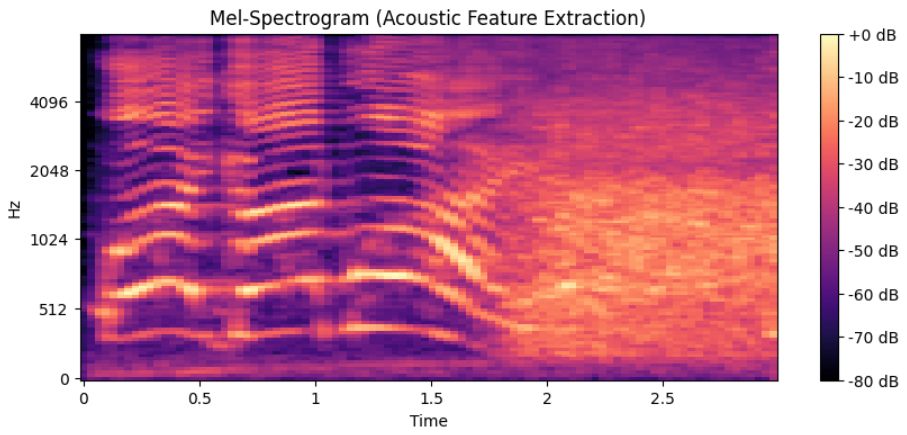
\includegraphics[width=0.7\textwidth]{images/mel_spectrogram.png}
    \caption{Mel-Spectrogram of a 3-second hook, used to extract MFCCs.}
    \label{fig:mel_spectrogram}
\end{figure}

 Figure  \ref{fig:mel_spectrogram} visualizes the Mel‑Spectrogram, which represents how energy is distributed across perceptual frequency bands over time. From this representation, we compute Mel‑Frequency Cepstral Coefficients (MFCCs), a compact descriptor widely used in speech and audio classification. MFCCs capture vocal timbre, clarity, and articulation patterns, helping the model distinguish between engaging speech, background noise, music, or muffled audio—key factors influencing perceived quality and retention.

\subsection{Semantic Profiling (LLM Zero-Shot)}
The LLM generates a structured semantic profile from the Whisper transcript by assigning a dominant tone category (e.g., educational, humorous, inspirational) and extracting high‑level intent signals. These labels convert unstructured language into categorical variables that are later one‑hot encoded. The distribution in the figure indicates which narrative styles dominate the dataset and provides interpretability: the model can be traced to psychological framing choices rather than only low‑level audiovisual patterns.

\begin{figure}[H]
    \centering
    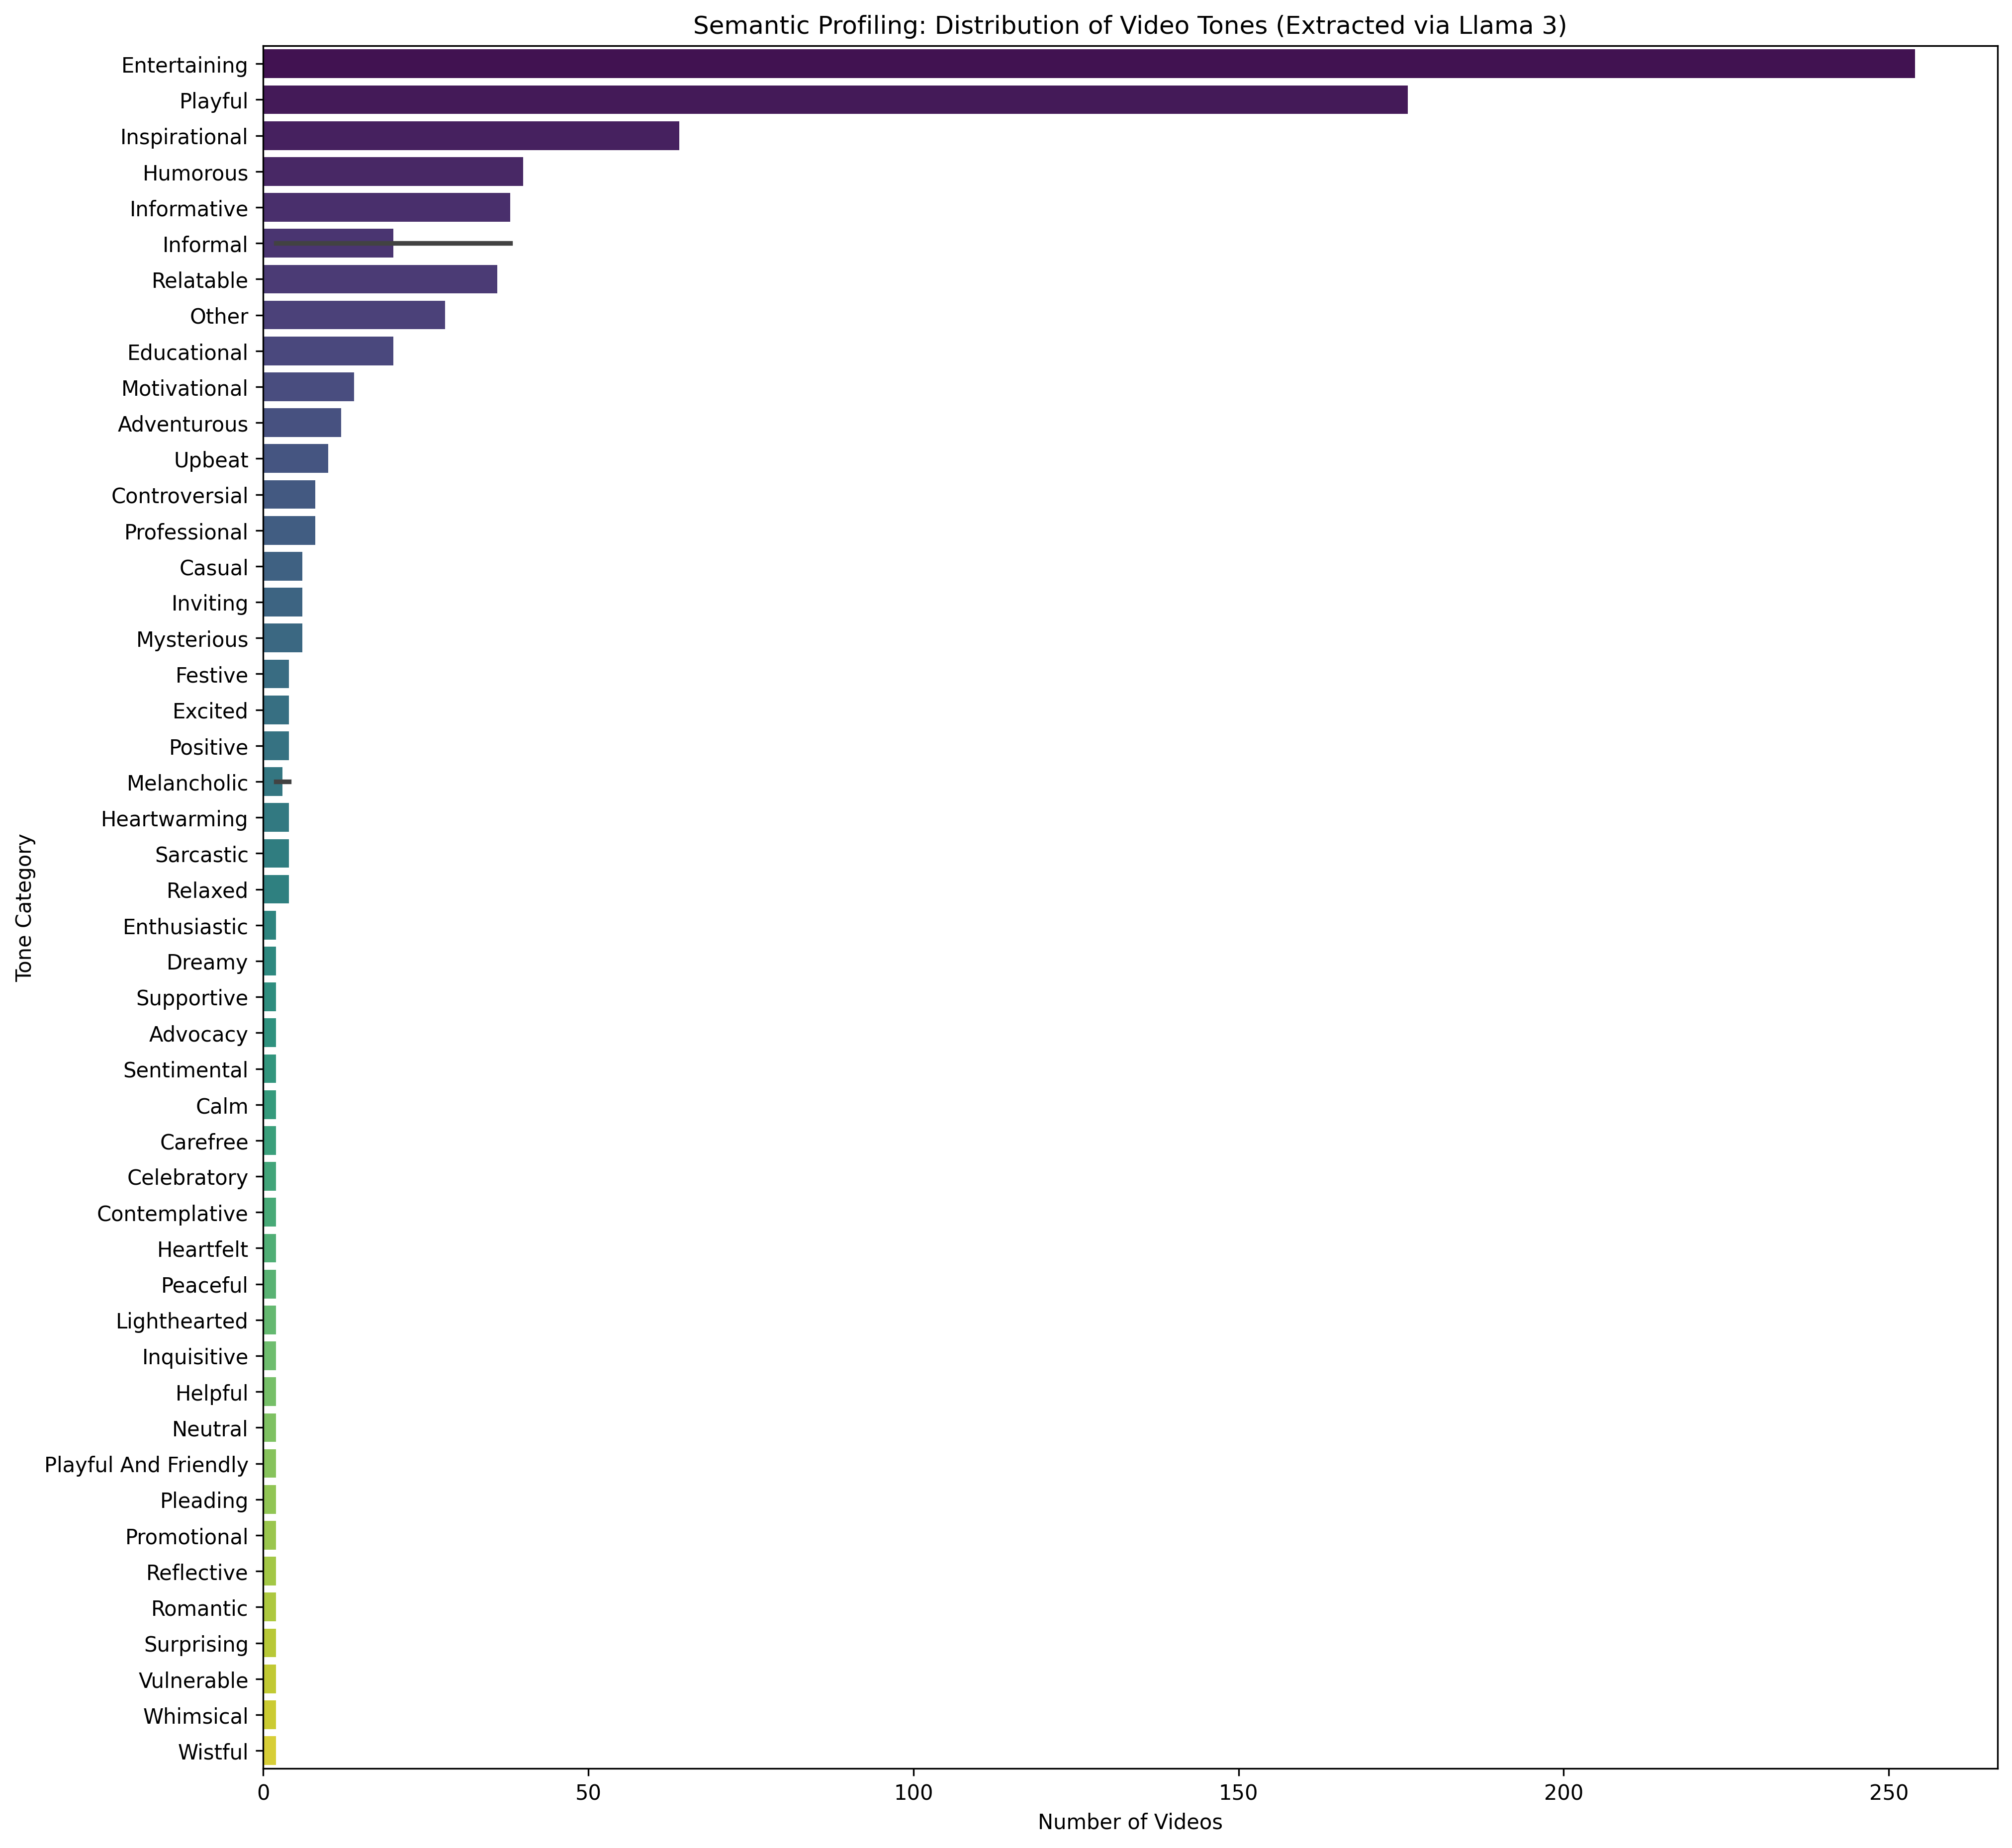
\includegraphics[width=0.75\textwidth]{images/llm_tone_distribution.png}
    \caption{Distribution of video tones extracted via Llama 3 semantic profiling.}
    \label{fig:llm_tone}
\end{figure}

\subsection{Speech-to-Text and Captioning Pipeline}
To maximize accessibility and engagement, we built a transcription and captioning module powered by Whisper. Audio is extracted as 16 kHz mono WAV, and \texttt{faster-whisper} generates word‑level timestamps. Captions are exported as SRT and then converted to ASS for advanced styling, including dynamic font scaling based on word length to ensure readability on 9:16 vertical videos. The final captions are burned into the video using FFmpeg, producing social‑ready, accessibility‑friendly content.

\subsection{Dimensionality Reduction (PCA)}
OpenAI CLIP produces 512‑dimensional embeddings for every video segment. While this rich representation captures fine‑grained visual semantics, it is too high‑dimensional for our dataset and would cause the model to overfit noise instead of learning general patterns.\\  We therefore apply Principal Component Analysis (PCA), which projects the embeddings into a lower‑dimensional subspace that preserves maximal variance. This reduces complexity, improves generalization, and significantly lowers computational cost without discarding the most informative visual signals.

\begin{figure}[H]
    \centering
    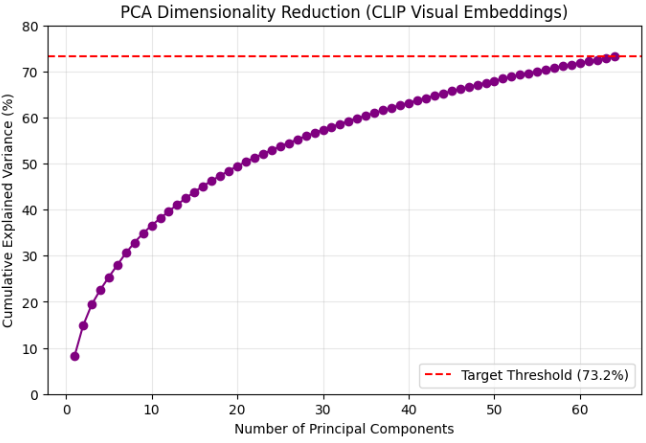
\includegraphics[width=0.6\textwidth]{images/pca_elbow_curve.png}
    \caption{PCA Cumulative Explained Variance for CLIP visual embeddings.}
    \label{fig:pca_elbow}
\end{figure}

Figure \ref{fig:pca_elbow} shows the cumulative explained variance of PCA applied to 512‑D CLIP embeddings. The curve rises quickly in the first components and gradually flattens, indicating diminishing returns. Selecting 64 components preserves approximately 73.4\% of the original variance, which is a strong trade‑off between compression and information retention. This reduces the risk of overfitting on a relatively small dataset while still keeping the most informative visual signals.\\

After dimensionality reduction, we also computed the cosine similarity between hook and full‑video embeddings to quantify visual consistency across the clip.

\begin{figure}[H]
    \centering
    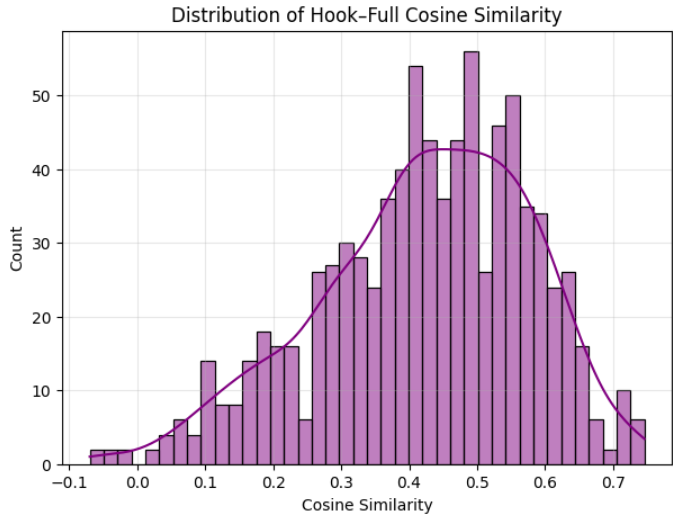
\includegraphics[width=0.6\textwidth]{images/hook_full_cosine_distribution.png}
    \caption{Distribution of cosine similarity between hook and full-video CLIP embeddings.}
    \label{fig:hook_full_cosine}
\end{figure}

Figure \ref{fig:hook_full_cosine} presents the distribution of cosine similarity between hook and full‑video embeddings. Most videos cluster around 0.4–0.6, meaning their opening visual style is moderately consistent with the rest of the content. Low similarity suggests that the hook does not match the main video, which may harm viewer retention, while very high similarity indicates strong visual coherence.
% ══════════════════════════════════════════════════════════════
\subsection{Preprocessing and Feature Engineering Design}

Data preprocessing is heavily customized for multimedia files:
\begin{itemize}
    \item \textbf{Multimodal Slicing:} Raw \texttt{.mp4} videos are programmatically separated into an audio track (\texttt{16kHz} mono \texttt{.wav} for Whisper/Librosa) and visual frames (\texttt{ffmpeg \%06d.png} format). For the predictive agent, the video is further sliced into the "Hook" (first 3 seconds) and the "Full Video" to independently assess user retention strategies.
    \item \textbf{Feature Aggregation:} The predictive agent aggregates the PCA vectors, Llama 3 categorical tags (One-Hot Encoded), and Librosa acoustic metrics into a flat, 473-dimensional dense matrix. 
    \item \textbf{Computer Vision Pre-Filtering:} Before passing frames to the heavy GANs, the system calculates Laplacian variance (blur) and Gaussian deltas (noise). Based on these thresholds, frames are routed through classical OpenCV filters (e.g., Bilateral Filtering with \texttt{d=9, sigma=75}) to remove digital artifacts, ensuring the GANs upscale clean data.
\end{itemize}
\subsection{AI Video Enhancement Pipeline (Optional Module)}
Although the core contribution is prediction, we implemented a separate AI enhancement pipeline to improve video quality before publishing. Each uploaded video is decomposed into frames and audio using FFmpeg. A quality analyzer measures blur (Laplacian variance), noise, and low‑light percentage across sampled frames. Based on these scores, the system auto‑selects a classical filter (bilateral or unsharp mask) to remove artifacts before AI restoration.

The enhancement stage applies a two‑model cascade: (1) Real‑ESRGAN for super‑resolution and texture reconstruction, and (2) GFPGAN for facial restoration when faces are detected. Enhanced frames are reassembled into an H.264 video using CRF‑18 and \texttt{-movflags +faststart} for immediate web playback. The pipeline also computes objective metrics (PSNR, SSIM, LPIPS) to quantify improvement and generates before/after previews for creators.
\subsection{Hyperparameter Configuration}

The models were fine-tuned to balance computational speed and output quality:

\begin{itemize}
    \item \textbf{Predictive Agent (XGBoost \& PCA):} The visual embeddings from CLIP (512D) and NLP embeddings from MiniLM (384D) were compressed using PCA with \texttt{n\_components} set to 64 and 48, respectively. The XGBoost regressor was configured with \texttt{learning\_rate = 0.05}, \texttt{max\_depth = 6}, and \texttt{n\_estimators = 200} to prevent overfitting while maintaining high predictive accuracy.
    \item \textbf{Auto-Captioning (Whisper):} The engine utilizes the \texttt{small} model size, balancing transcription accuracy with processing speed. The \texttt{beam\_size} is set to 5 for optimal decoding, and \texttt{word\_timestamps=True} is strictly enforced to enable dynamic, word-by-word subtitle flashing.
    \item \textbf{Video Enhancement:} Real-ESRGAN is configured with \texttt{scale=4} for ultra-HD upscaling, utilizing a \texttt{tile=512} and \texttt{tile\_pad=10} strategy to prevent GPU Out-Of-Memory (OOM) errors on high-resolution frames. GFPGAN runs on \texttt{version=1.4}. FFmpeg encoding uses a Constant Rate Factor (\texttt{CRF}) of 18 and \texttt{-movflags +faststart} to ensure the final output is pristine and instantly streamable on the web.
\end{itemize}
\section{Model Training and Results}
% ══════════════════════════════════════════════════════════════

The dataset was divided using an 80/20 Train/Test split, ensuring strict deduplication based on \texttt{video\_id} to prevent data leakage. We evaluated multiple models using RMSE, MAE, and $R^2$ scores.

\subsection{Model Choice and Selection Rationale}
To ensure robustness, we compared three strong tree-based regressors widely used for structured, high-dimensional data:
\begin{itemize}
    \item \textbf{XGBoost (XGB):} Known for excellent generalization and strong performance on mixed numerical + categorical features.
    \item \textbf{LightGBM (LGBM):} Optimized for speed and large feature spaces, often competitive with XGBoost.
    \item \textbf{Random Forest (RF):} A reliable baseline ensemble with low variance but weaker performance on complex interactions.
\end{itemize}
To formally evaluate model performance, we computed standard regression metrics defined as follows:

\noindent
\begin{minipage}{0.48\textwidth}
\begin{equation}
\text{MAE} = \frac{1}{n}\sum_{i=1}^{n} \left| y_i - \hat{y}_i \right|
\end{equation}
\end{minipage}
\hfill
\begin{minipage}{0.48\textwidth}
\begin{equation}
\text{RMSE} = \sqrt{ \frac{1}{n}\sum_{i=1}^{n} \left( y_i - \hat{y}_i \right)^2 }
\end{equation}
\end{minipage}

\begin{equation}
R^2 = 1 - \frac{\sum_{i=1}^{n} (y_i - \hat{y}_i)^2}{\sum_{i=1}^{n} (y_i - \bar{y})^2}
\end{equation}

MAE captures average absolute error, RMSE penalizes large deviations, and $R^2$ measures the proportion of variance explained by the model.

\begin{table}[H]
    \centering
    \begin{tabular}{lccc}
        \toprule
        \textbf{Model} & \textbf{RMSE} & \textbf{MAE} & \textbf{$R^2$ Score} \\
        \midrule
        XGBoost (Selected) & \textbf{0.83} & \textbf{0.36} & \textbf{0.85} \\
        LightGBM & 0.90 & 0.42 & 0.82 \\
        Random Forest & 1.12 & 0.78 & 0.73 \\
        \bottomrule
    \end{tabular}
    \caption{Performance comparison of regression models predicting \texttt{log\_views}.}
    \label{tab:model_comparison}
\end{table}

\begin{figure}[H]
    \centering
    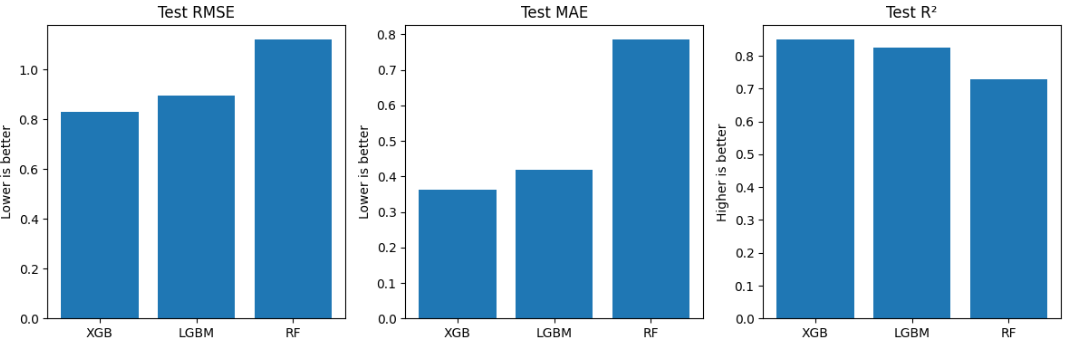
\includegraphics[width=0.9\textwidth]{images/model_comparaison_bars.png}
    \caption{Test set comparison of RMSE, MAE, and $R^2$ across XGBoost, LightGBM, and Random Forest.}
    \label{fig:model_comparison_bars}
\end{figure}

Table \ref{tab:model_comparison}  and Figure \ref{fig:model_comparison_bars}  provide a comparative evaluation across three ensemble models. Although all three perform reasonably well, XGBoost consistently achieves the lowest RMSE and MAE while also delivering the highest $R^2$ score.
\\ LightGBM follows closely but remains inferior in both error metrics, while Random Forest exhibits significantly higher error and lower explanatory power. \\
XGBoost achieved the lowest error and highest $R^2$, making it the most reliable model for deployment. The performance gap is also visible in Figure \ref{fig:model_comparison_bars}, where XGBoost consistently dominates across all three metrics.
\subsection{Results}

\begin{figure}[H]
    \centering
    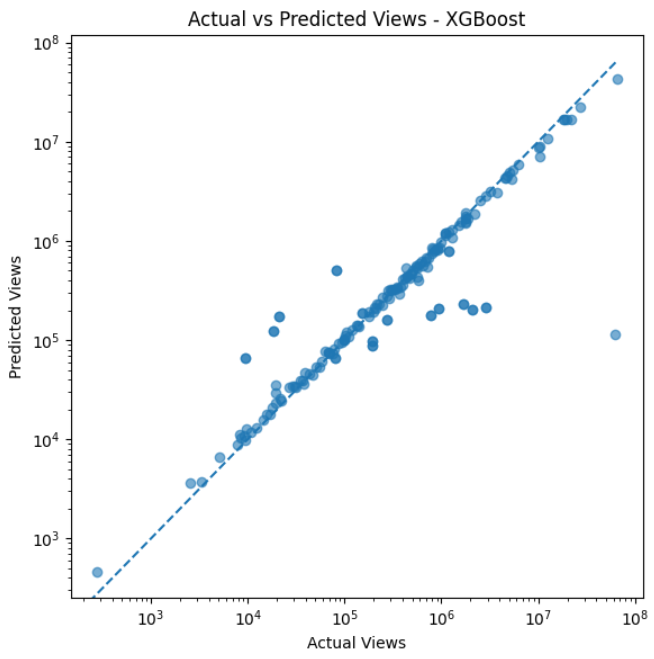
\includegraphics[width=0.4\textwidth]{images/actual_vs_predicted.png}
    \caption{XGBoost Regression Fit: Actual vs. Predicted \texttt{log\_views}.}
    \label{fig:actual_vs_predicted}
\end{figure}

The few deviations from the diagonal correspond to rare viral outliers, which are influenced by external platform dynamics not directly encoded in the video content. Overall, the tight clustering confirms the model’s strong predictive reliability.

% ══════════════════════════════════════════════════════════════
\section{Diagnostics and Explainability}
% ══════════════════════════════════════════════════════════════

\subsection{Learning and Loss Curves}
To prove the model's stability and validate our hyperparameter choices, we generated learning curves and loss curves.

\begin{figure}[H]
    \centering
    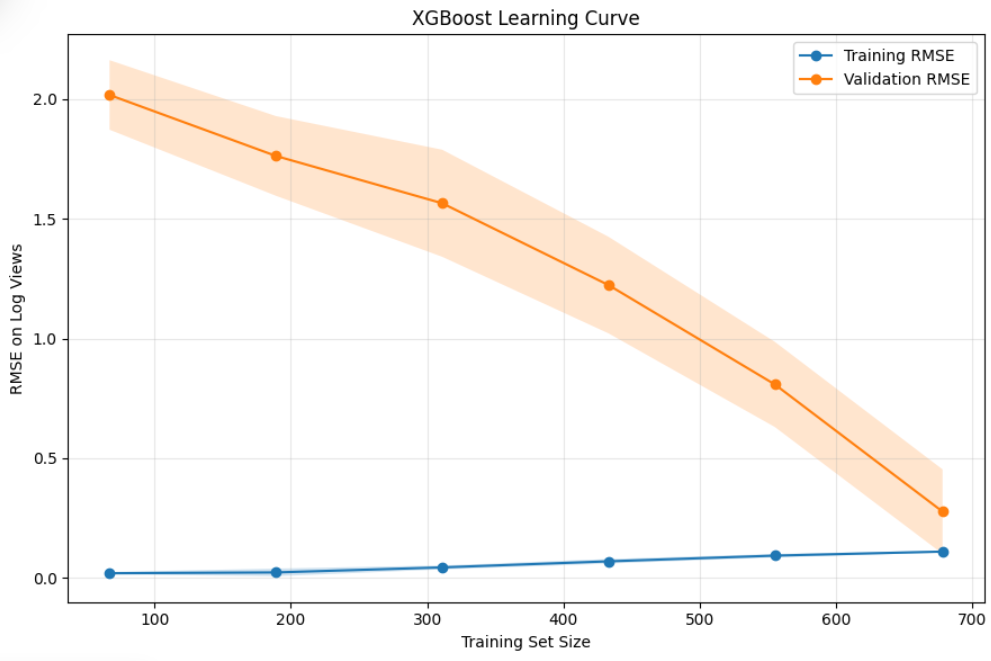
\includegraphics[width=0.6
    \textwidth]{images/learning_curve.png}
    \caption{XGBoost Learning Curve over increasing dataset sizes.}
    \label{fig:learning_curve}
\end{figure}
Figure \ref{fig:learning_curve}  shows a clear generalization trend. The validation RMSE drops consistently as the training size increases, which proves that model performance is data-limited rather than architecture-limited. The shaded band (variance) narrows with larger datasets, indicating reduced sensitivity to sample selection. This confirms that the dataset size is sufficient to stabilize XGBoost and that adding more data directly improves predictive reliability.
\begin{figure}[H]
    \centering
    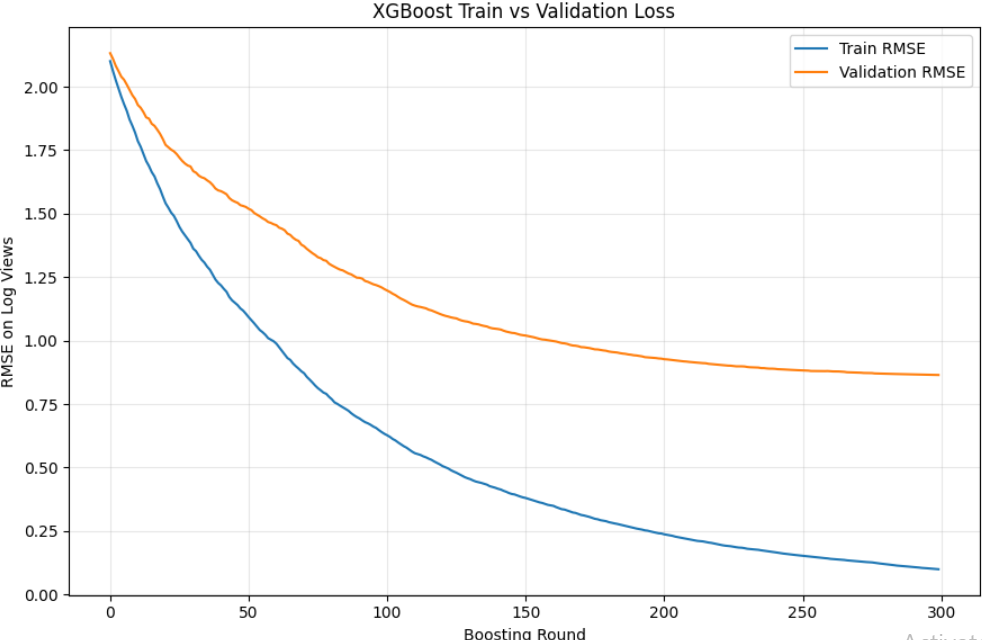
\includegraphics[width=0.6\textwidth]{images/training_loss.png}
    \caption{XGBoost Loss Curve over 300 boosting rounds.}
    \label{fig:training_loss}
\end{figure}

Figure \ref{fig:training_loss} mathematically justifies our data collection efforts; the validation error plunges linearly as more data is introduced. Furthermore, Figure \ref{fig:training_loss} shows smooth convergence without a "U-shape", proving the model does not suffer from late-stage overfitting and justifying the \texttt{n\_estimators=300} limit.
\subsection{Model Explainability (SHAP)}
To provide actionable feedback to content creators, we applied TreeSHAP (SHapley Additive exPlanations), which computes the marginal contribution of each feature to a single prediction. Unlike global feature importance, SHAP explains \emph{why a specific video} is predicted to perform well or poorly by decomposing the final output into positive and negative feature attributions.

In practice, this allows BViral to generate human‑readable advice such as “reduce silence in the first seconds” or “increase hook energy.” It also validates that the model is relying on meaningful signals (e.g., hook embeddings, acoustic energy, and LLM tone categories) rather than spurious correlations. This explainability layer is critical for creator trust and converts the model from a black‑box predictor into a decision‑support agent.

% ══════════════════════════════════════════════════════════════
\section{Critical Discussion \& Architectural Pivot}
% ══════════════════════════════════════════════════════════════
Initially, the project scope included a "Post-Posting" model to predict Engagement Rate. However, our experiments yielded a poor $R^2$ score (0.36) for this metric. Analysis revealed that engagement is heavily influenced by latent external noise (e.g., creator follower count, algorithmic randomization, and time of day) that cannot be extracted from a raw \texttt{.mp4} file. 

Consequently, we made the strategic Data Science decision to drop the Post-Posting model. By scoping down, we focused all compute resources on perfecting the highly reliable \textbf{Pre-Posting Predictive Agent}, ensuring BViral remains a professional, deterministic SaaS tool rather than relying on noisy, uncontrollable post-publication metrics.

\section{Future Improvements}
A major future direction is scaling the dataset. Larger datasets would increase model generalization but require heavier compute resources for feature extraction (CLIP, Whisper, LLM). Future work will therefore allocate stronger GPU/CPU hardware to prevent extraction crashes and to enable batch processing at scale. With more stable infrastructure, we can safely expand the dataset and retrain the model with richer multimodal coverage, potentially improving $R^2$ beyond the current results.
% ══════════════════════════════════════════════════════════════
\section*{Conclusion}
\phantomsection
\addcontentsline{toc}{section}{Conclusion}
% ══════════════════════════════════════════════════════════════
This chapter exhaustively validated the AI methodologies powering BViral Control Center. Through rigorous EDA and the visualization of our multimodal pipeline (PCA, Audio Spectrograms, LLM classification), we proved the complexity of our feature extraction. The XGBoost model successfully mapped these 473 features to achieve an $R^2$ of 0.85, while SHAP integration provided the essential explainability required for a creator-facing agent.